%%
%% This is file `sample-sigconf.tex',
%% generated with the docstrip utility.
%%
%% The original source files were:
%%
%% samples.dtx  (with options: `sigconf')
%%
%% IMPORTANT NOTICE:
%%
%% For the copyright see the source file.
%%
%% Any modified versions of this file must be renamed
%% with new filenames distinct from sample-sigconf.tex.
%%
%% For distribution of the original source see the terms
%% for copying and modification in the file samples.dtx.
%%
%% This generated file may be distributed as long as the
%% original source files, as listed above, are part of the
%% same distribution. (The sources need not necessarily be
%% in the same archive or directory.)
%%
%% The first command in your LaTeX source must be the \documentclass command.
\documentclass[conference]{IEEEtran}
%% IEEE CNS addition:
\makeatletter
\def\ps@headings{%
\def\@oddhead{\mbox{}\scriptsize\rightmark \hfil \thepage}%
\def\@evenhead{\scriptsize\thepage \hfil \leftmark\mbox{}}%
\def\@oddfoot{}%
\def\@evenfoot{}}
\makeatother
\pagestyle{empty}

\usepackage[utf8]{inputenc}
\usepackage{multirow}
\usepackage[inline]{enumitem}
\usepackage{xcolor}
\usepackage{booktabs}
\usepackage{hyperref}
\usepackage{amsmath}
\usepackage{amssymb}
\usepackage{graphicx}
\usepackage[numbers]{natbib}
\usepackage{subfig}

\usepackage[nomain, toc, acronym]{glossaries}
\glsdisablehyper

\newcommand\note[2]{{\color{#1}#2}}
\newcommand\todo[1]{{\note{red}{TODO: #1}}}

% Adds a "given" symbol (vertical bar) that rescales in height (like \left and \right)
\usepackage{mathtools}
\newcommand\givenbase[1][]{\:#1\lvert\:}
\let\given\givenbase
\newcommand\sgiven{\givenbase[\delimsize]}
\DeclarePairedDelimiterX\Basics[1](){\let\given\sgiven #1}
\newcommand\Average{E\Basics}

%%
%% end of the preamble, start of the body of the document source.
\begin{document}

%%
%% The "title" command has an optional parameter,
%% allowing the author to define a "short title" to be used in page headers.
\title{SparseIDS: Learning Packet Sampling with Reinforcement Learning}

\author{\IEEEauthorblockN{Maximilian Bachl, Fares Meghdouri, Joachim Fabini, Tanja Zseby}
\IEEEauthorblockA{Technische Universität Wien\\
firstname.lastname@tuwien.ac.at}}

%\date{\today}

% \IEEEoverridecommandlockouts
% \IEEEpubid{\begin{minipage}[t]{\textwidth}\ \\[10pt]
%         \centering\normalsize{xxx-x-xxxx-xxxx-x/xx/\$31.00 \copyright 2018 IEEE}
% \end{minipage}}

% \renewcommand*{\bibfont}{\footnotesize}

\maketitle%

%\thispagestyle{plain}
%\pagestyle{plain}

\newacronym{ml}{ML}{Machine Learning}
\newacronym{dl}{DL}{Deep Learning}
\newacronym{aml}{AML}{Adversarial Machine Learning}
\newacronym{ids}{IDS}{Intrusion Detection System}
\newacronym{rnn}{RNN}{Recurrent Neural Network}
\newacronym{fgsm}{FGSM}{Fast Gradient Sign Method}
\newacronym{cw}{CW}{Carlini-Wagner method}
\newacronym{pgd}{PGD}{Projected Gradient Descent}
\newacronym{pdp}{PDP}{Partial Dependence Plot}
\newacronym{ars}{ARS}{Adversarial Robustness Score}
\newacronym{ttl}{TTL}{Time-to-Live}
\newacronym{dos}{DoS}{Denial-of-Service}
\newacronym{iat}{IAT}{Interarrival time}
\newacronym{rl}{RL}{Reinforcement Learning}
\newacronym{dpi}{DPI}{Deep Packet Inspection}
\newacronym{ac}{AC}{Actor-Critic}

\newcommand{\ours}{SparseIDS}

\begin{abstract}

\glspl{rnn} have been shown to be valuable for constructing \glspl{ids} for network data. They allow analyzing network flows and already determining if a flow is malicious or not before it is over, making it possible to take action immediately. However, considering the large number of packets that have to be inspected, the question of computational as well as energy efficiency arises. We show that by using a novel \gls{rl}-based approach called \textit{\ours{}}, we can reduce the number of consumed packets by more than three fourths while keeping classification accuracy high. Comparing to various other sampling techniques, \ours{} consistently achieves higher classification accuracy with the same number of sampled packets. A major novelty of our \gls{rl}-based approach is that it can not only skip up to a predefined maximum number of packets like current approaches but can possibly skip arbitrarily many packets, saving even more computational resources for long sequences. Finally we build an automatic steering mechanism that can guide \ours{} to achieve a desired level of sparsity. 

\end{abstract}

%%
%% The abstract is a short summary of the work to be presented in the
%% article.
%\begin{abstract}
%  A clear and well-documented \LaTeX\ document is presented as an
%  article formatted for publication by ACM in a conference proceedings
%  or journal publication. Based on the ``acmart'' document class, this
%  article presents and explains many of the common variations, as well
%  as many of the formatting elements an author may use in the
%  preparation of the documentation of their work.
%\end{abstract}

\maketitle

\section{Introduction}
\label{sec:introduction}

There is a significant body of scientific work focusing on the detection of unwanted behavior in networks. In the past, a viable way of performing intrusion detection was to inspect the content of packets themselves and detect if a packet delivers potentially harmful content. More recently, with the increasing deployment of encryption, the focus now lies on features that are always available to network monitoring equipment like port numbers, protocol flags or packet sizes when encrypting above the transport layer.

% Fares:
%As the need for security mechanisms in today's infrastructure communication networks grows, a substantial body of scientific work focuses on developing reliable, explainable frameworks for the identification of unwanted behaviors. In the past, a viable way to detect intrusion was to analyze the contents of the packets themselves and determine, for example, whether a packet contains potentially harmful content by matching patterns. More recently, with the increasing deployment of encryption, the focus is now on features that are always available for network monitoring devices such as port numbers, protocol flags, packet sizes when encrypting above the transport layer.

Network communication is usually aggregated into \textit{flows}, which are commonly defined as a sequence of packets sharing certain properties. When analyzing flows, not only the aforementioned features are available but also features related to the timing of the individual packets. Various approaches have been proposed to extract features from flows and then perform anomaly detection with the extracted flows \cite{meghdouri_analysis_2018}.
While these approaches frequently work well, it is problematic that the whole flow has to be received first and only afterwards anomaly detection is applied, revealing attack flows. Thus, we design a network \gls{ids} that operates on a per-packet basis and decides if a packet is anomalous based on features that are available even for traffic that is encrypted above the transport layer, like for example TLS or QUIC.
At the same time, an \gls{rnn}-based \gls{ids} has the benefit of avoiding tedious feature engineering procedures, which derive statistical measures from the sequence of packet features, but providing any available information to the classifier.
\cite{hartl_explainability_2019} showed that such a system has similar performance to other flow-based anomaly detection systems but can detect anomalies \textit{before} the flow terminates and analyzed its security with respect to adversaries extensively. 

% Fares:
%A network communication is typically aggregated into \textit{flows}, which are commonly defined as a sequence of packets that share certain properties. When analyzing flows, not only the aforementioned features are available but also features representing the temporal behavior of the individual packets. Various approaches have been proposed to extract flows features after which anomaly detection can be performed, in \cite{meghdouri_analysis_2018} Meghdouri et al. compare such approaches.
%While these approaches often work well, it is troublesome because, in the worst case, the whole flow must be received first and only then anomaly detection can be applied; revealing malicious flows. Thus, we design a network \gls{ids} that operates on a per-packet basis and determines whether packet is anomalous based on features that are available even for traffic that is encrypted above the transport layer, like for example TLS or QUIC.
%At the same time, an \gls{rnn}-based \gls{ids} has the benefit of avoiding tedious feature engineering procedures, which derive statistical measures from the sequence of packet features, but providing any available information to the classifier.
%In \cite{hartl_explainability_2019}, Hartl et al. show that such an architecture has similar performance to other flow-based anomaly detection systems, but can still detect anomalies \textit{before} the flow ends and analyzed its robustness with respect to adversaries extensively. 

However, for practical use, not only classification accuracy and security are important but also computational efficiency. This follows from the fact that a rationally-acting company will only deploy an \gls{ids} if the cost that is saved by avoiding security breaches is higher than the cost of the \gls{ids} itself. The cost of the \gls{ids} can be split in the cost of purchase/installation, the cost of operating it and the cost of maintaining it. The goal we pursue here is to develop sampling strategies that do not significantly degrade classification performance while being able to only process a small fraction of the original data. Specifically, the sampling technique should

% Fares:
%Nevertheless, not only the accuracy and reliability of classification, but also the computational efficiency, are critical for practical use. This follows from the fact that a rationally-acting organization will only implement an \gls{ids} if the cost saved by preventing security breaches is higher than the cost of the \gls{ids} itself. Noteworthy that the cost of an \gls{ids} can be divided into (a) the cost of purchase/installation, (b) the cost of operation and (c) the cost of maintenance.  The goal we pursue here is to develop autonomous sampling strategies that do not significantly degrade classification performance while being able to only process a small fraction of the original data. Specifically, the sampling technique should:

\begin{enumerate}
\item \textbf{choose optimally}, taking only the data that contain the most information and skip the less relevant ones. 
% Fares:
%\item \textbf{choose optimally}, taking only samples that contain the most information and skip the less relevant ones. 
\item have a parameter that allows to \textbf{trade off} classification performance for sparsity.
\item be \textbf{independent of the classifier} so that any classifier can be used and that the classifier doesn't have to be aware of the sampling strategy. 
\item be \textbf{retrainable} so that the sampling can be continuously adapted depending on the current threat landscape. 
\item be able to \textbf{skip arbitrarily} many packets since network flows can be very long but only the first couple of packets are needed to decide whether an attack occurred or not and the remaining packets can be skipped altogether. 
\end{enumerate}


For this purpose, we develop the \gls{rl}-based \gls{ids} \textit{\ours{}} fulfills the above properties. We show that a significant number of packets can be skipped while accuracy doesn't drop significantly. Compared to other common sampling strategies, \ours{} performs better when being trained on the same number of packets. 

% Fares:
%For this purpose we develop a \gls{rl}-based \gls{ids}: \textit{\ours{}} that fulfills the above properties. We show that a significant number of packets can be skipped while the accuracy does not drop
%considerably. Compared to other common sampling techniques, \ours{} performs better when being trained on the same number of packets.

As \ours{} uses a parameter to trade-off accuracy for sparsity, the resulting accuracy and sparsity are determined by this parameter. However, since it also might be desired to specify the sparsity itself, we propose a steering system which takes a desired sparsity as its input and modifies the parameter of the reinforcement learning in a control loop until the specified sparsity is reached. 

% Fares:
%The accuracy-sparsity trade-off of \ours{} can be regulated by a reinforcement learning parameter that directly affects both later quantities. However, in certain situations, a certain sparsity is to be achieved, hence we further develop and propose a steering system that fluctuates such a trade-off parameter in order to obtain a coveted sparsity in a closed control loop.

To encourage reproducibility and facilitate experimentation, we publicly release the source code, the data and the figures of this work at \url{https://github.com/CN-TU/adversarial-recurrent-ids/tree/rl}

\section{Related Work}

\cite{hartl_explainability_2019} build an LSTM-based recurrent classifier for Network Intrusion Detection and develop methods for explainability and to assess the security of recurrent classifiers. 

\cite{yu_learning_2017} propose using \gls{rl} to let an LSTM learn to skim text. Their technique does not aim to maximize sparsity but only lets the \gls{rl} optimize classification performance for the sequence as a whole. Thus, if it learns to skip elements it is only because it is better for achieving good classification performance, not because it wants to increase sparsity. 

\cite{campos_skip_2018} develop a technique that includes a \textit{skip gate} into LSTM or GRU \todo{citation needed} cells. It works without \gls{rl} but on the downside, their method can only be trained once and not be adapted afterwards and also it explicitly depends on the the implementation of the underlying classifier, while we want to be independent of it. 

\cite{seo_neural_2018} use an LSTM with one full state vector and one reduced one. At each step they decide whether to use the reduced or the full state vector and can reduce computational cost by using the reduced one. For network traffic we think that it is often not even necessary to have a reduced state vector since from some attack flows, already the first couple of packets might contain enough information and then the remaining packets of the flow do not have to be considered anymore at all. 

\cite{gui_long_2018} use \gls{rl} but their intention is not to skip samples but instead to make the \gls{rl} learn to choose a previous state that can aid at the current step. Thus it tries to help the \gls{rnn} with memorizing information from the past but does not actually take less data, which is the goal we pursue in this work. 

These proposed techniques focus their evaluation on text and hence do not fulfill certain criteria we set out in \autoref{sec:introduction}. Furthermore, all techniques that use \gls{rl} use discrete actions, meaning that there is a hyperparameter $k$, which influences the maximum jump that is possible. However, for a network flow, already after the second packet it might be obvious that a flow is an attack and thus the remaining packets can be completely ignored. It is thus beneficial to not have a fixed maximum step size but a continuous one. 

%\section{Setup}
%%ci
\section{Classifier}
\label{sec:classifier}
We implemented a three-layer LSTM-based classifier with 128 neurons at each layer. As the input features we use source port, destination port, protocol identifier, packet length, \gls{iat} to the previous packet in the flow, packet direction (i.e. forward or reverse path) and all TCP flags (0 if the flow is not TCP).
We omitted \gls{ttl} values, as they are likely to lead to unwanted prediction behaviour \cite{bachl_walling_2019}.  Among the used features, source port, destination port and protocol identifier are constant over the whole flow while the others vary.
Additionally, we add the number of skipped packets since the last packet as a feature, which can help the classifier because otherwise it might be confused because of missing packets. 
During flow extraction we used the usual 5-tuple flow key, which distinguishes flows based on the protocol they use and their source and destination port and IP address.
We use Z-score normalization and a train/test split of 2:1.

\section{RL for Sampling}
\label{sec:rlForSampling}
Given enough training instances, \gls{rl} algorithms have been shown to perform very well in complex decision-making situations such as playing video games \cite{mnih_playing_2013} as well as networking problems such as congestion control \cite{bachl_rax_2019}. We thus consider an \gls{rl}-based architecture to be suitable for taking packet sampling decisions. The system should look at the current packet as well as the history of the conversation flow and output how many packets should be skipped until the next packet is considered in the current flow. The reward that the \gls{rl} tries to maximize should be a combination of classification accuracy and the number of packets that could be skipped (sparsity). An operator should be able to specify how much accuracy is allowed to be traded off for achieving higher sparsity.% and the objective of the \gls{rl} at a timestep t of a flow is defined as:

%\begin{align}
%\begin{split}
%U_t = & \text{future average classification performance} \\
%+ & \alpha\times\text{future average sparsity}
%\end{split}
%\end{align}

For a flow of length $T$ at each timestep $t$ we have two reward metrics which we compute in a fashion that is known from \textit{R-learning} \cite{schwartz_reinforcement_1993}:

\begin{figure}
\centering
  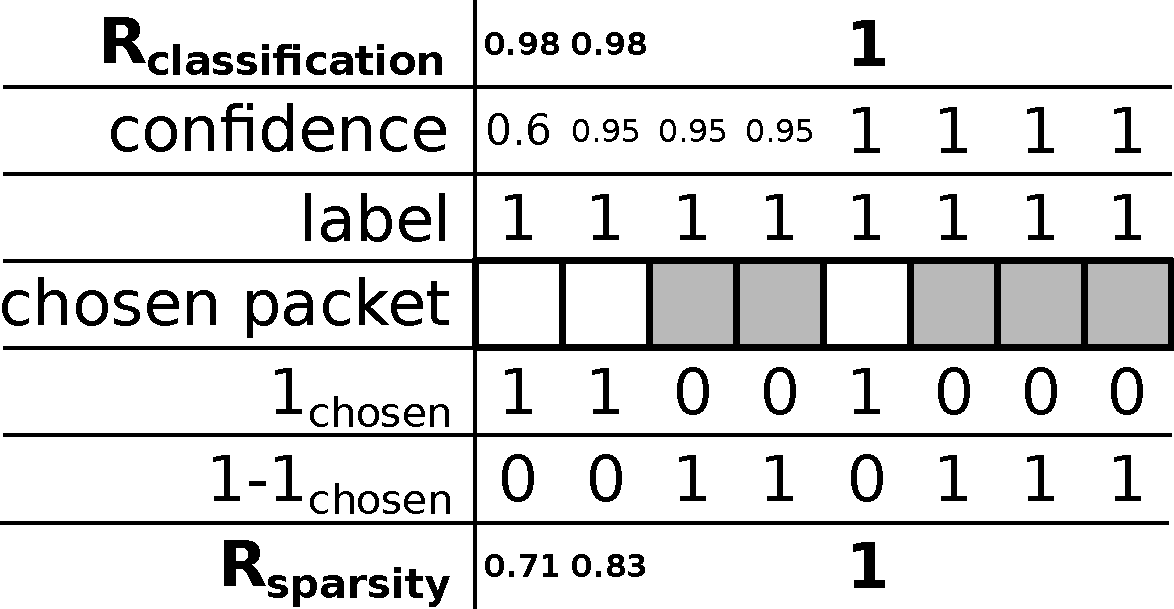
\includegraphics[width=\columnwidth]{img/rewards.pdf}
  \caption{The computation of the rewards for a sample flow: Gray packets are skipped while white ones are chosen. At the top row the resulting rewards for classification for each chosen packet are depicted and in the bottom row the ones for sparsity. Numbers are rounded to two digits after the decimal point.}
  \label{fig:rewards}
\end{figure}

The classification reward metric captures how correct the classifier is on average for all future packets of a flow. The label of each packet in a flow has a value of 0 for non-attack traffic and 1 for attack traffic with one flow being only attack or non-attack but not mixed. The confidence is the sigmoided ($\frac{e^x}{1+e^x}$) output of the classifier, yielding a value between 0 and 1, where 0 is absolute confidence for a flow being benign and 1 is absolute confidence for a flow being an attack. 
\begin{align}
\begin{split}
R_{\text{classification},t} = \frac{1}{T-t} \sum_{i=t+1}^{T} |\text{label}_t - \text{confidence}_t|
\end{split}
\end{align}

The sparsity reward metric captures how much sparsity is achieved on average for all future packets of a flow. E.g. for a flow of length 10 if after timestep 5, 3 packets are chosen and 2 are skipped, the sparsity reward metric at timestep 5 is $\frac{2}{2+3}=\frac{2}{5}$.
\begin{align}
\begin{split}
R_{\text{sparsity},t} = \frac{\sum_{i=t+1}^{T} 1_{\text{skipped},t}}{\sum_{i=t+1}^{T} 1_{\text{chosen},t}+\sum_{i=t+1}^{T} 1_{\text{skipped},t}}
\end{split}
\end{align}

We opt for an \emph{\gls{ac}} approach (as shown in \autoref{fig:sampling}) modeled after \cite{mnih_asynchronous_2016} because we consider it being more interpretable than a Deep \gls{rl} approach based on a \textit{Deep Q Network} like \cite{mnih_playing_2013} for reasons we explain later \todo{Max: Add ref to the section where we explain this}. 

Our proposed framework consists of three independent neural networks: the classifier, the critic and the actor. 

The classifier's goal is to guess correctly if a flow is an attack or not. For this, it outputs its confidence for non-attack/attack after reading a packet. As stated in \autoref{sec:classifier}, we choose an LSTM-based supervised classifier for this work, but our framework can work together with any classifier as long as it outputs a confidence for non-attack/attack at each timestep and can handle skipped packets. For instance it would also be possible to replace the LSTM with an unsupervised autoencoder like in \cite{mirsky_kitsune_2018}. 

The Critic aims to estimate the future expected average classification performance and the future expected average sparsity that can be achieved at a timestep $t$. For this it outputs $v_{\text{classification},t}$ and $v_{\text{sparsity},t}$ at each timestep $t$. It aims to predict the classification performance and sparsity correctly for each timestep by minimizing the following loss function:
\begin{align}
\begin{split}
l_{\text{v},t} =& \left(R_{\text{classification},t} - v_{\text{sparsity},t}\right)^2 + \left(R_{\text{sparsity},t} - v_{\text{sparsity},t}\right)^2
\end{split}
\end{align}

Now that the reward metrics and the Critic's outputs are defined, we can define the overall utility that we want to maximize at each timestep $t$ as follows:
\begin{align}
\begin{split}
U_t =& \left(R_{\text{classification},t} + \alpha \cdot R_{\text{sparsity},t}\right) \\
- & \left(v_{\text{classification},t} + \alpha \cdot v_{\text{sparsity},t}\right)
\end{split}
\end{align}

This means that we want that we want the reward to be higher than the Critic's expectation. 

The Actor outputs a probability distribution at timestep $t$, which is sampled to determine the number of packets that should be skipped. It aims to change the distribution so that actions which result in a higher reward are chosen more frequently, maximizing the utility function. However, this strategy could lead to the Actor getting stuck with what it considers the best decision and never try alternatives even though they might result in a higher reward. Thus, the Actor not only tries to change the distribution so that the actions become more optimal but at the same time also aims to maximize the entropy of the distribution so that alternative choices are still explored reasonably often. 

Specifically, at timestep $t$, given the current state $s_t$ (which consists of the current input as well as the LSTM state) and the neural network weights of the Actor $\theta_a$ the Actor outputs a probability distribution $\pi \left( a_t \given s_t ; \theta_\text{a} \right)$ from which the action $a_t$, the number of packets to be skipped, is sampled. Besides wanting to make actions which result in a high reward more likely, the actor also seeks to optimize the entropy $H(\cdot)$ of the probability distribution so that it keeps exploring and doesn't get stuck with a suboptimal policy. 

Combining these objectives, the actor network aims to minimize the loss function
\begin{align}
\begin{split}
l_{\text{a},t} =& -\log \left( \pi \left( a_t \given s_t ; \theta_\text{a} \right) \right) U_t \\ 
&- \beta H\left( \pi\left( s_t; \theta_a \right)\right)
\end{split}\label{eq:actor}
\end{align}

%The Critic network evaluates the behavior of the Actor network and computes the classification performance and sparsity that it thinks is going to be achieved.% using the computed value function and gives it feedback based on the performance obtained by the LSTM classifier. 
%The number of packets to skip is taken from the Actor's output distribution and fed into the packet parser, which is responsible for counting the packets and selecting the appropriate one.

In related work regarding \gls{rl}-based sampling for sequences, only discrete actions were evaluated so far: The actor would output a categorical probability distribution with a fixed maximum number of bins $k$. A drawback of this approach is that only a predefined maximum number of packets can be skipped and that that for a very large number of $k$, it can take a long time to converge to an optimum policy as there are $k$ different options to explore at each timestep $t$. Besides discrete actions, we thus also experiment with continuous actions, which allow to skip arbitrarily many packets. 

\begin{figure}
\centering
  \includegraphics[width=\columnwidth]{neural_network.pdf}
  \caption{An overview of the complete neural network being used in our experiments. Ocher stands for the input, blue for linear layers, red for LSTM layers and purple for the outputs of the neural network. The numbers in parentheses next to each label stand for the width of that layer (i.e.~the number of neurons (except for the inputs and outputs)). Parts of the neural network are shared between $v_\text{classification}$ and $v_\text{sparsity}$ as well as $\mu$ and $\sigma$ as they output quantities of similar magnitude and thus the gradients that are computed when updating the neural network are of the same order of magnitude as well. Our implementation also supports sharing the LSTM between all three neural network. However, as the five outputs can produce losses that have different order of magnitude, larger gradients or larger losses would ``overwrite'' the gradients of the smaller ones.}
  \label{fig:neuralNetworkArchitecture}
\end{figure}

An overview of the neural networks of the classifier, actor and critic that we use in this work is given in \autoref{fig:neuralNetworkArchitecture}.

\begin{figure}
\centering
  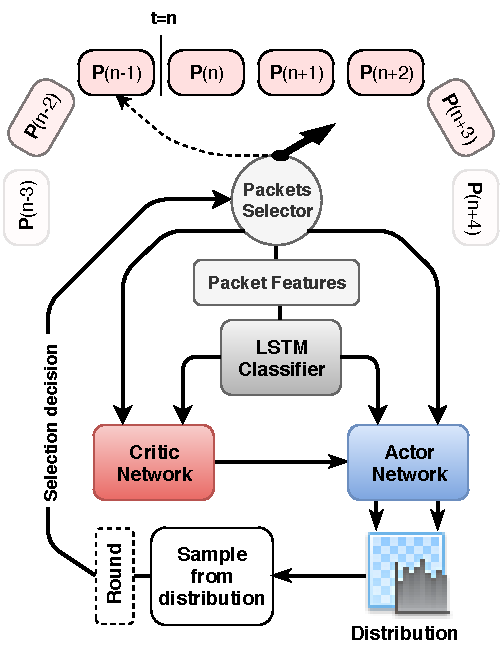
\includegraphics[width=\columnwidth]{img/rnn-sampling.pdf}
  \caption{SparseIDS framework. Three deep networks are shown: an LSTM classifier, An Actor network and a Critic network. The Actor takes actions based on the feedback from the the Critic network and the classifier. The Critic network tracks the Actor actions based on the classifier confidence and finally, the packets selector parses packets based on the decision of the Actor network.}
  \label{fig:sampling}
\end{figure}

A schematic overview over the \gls{rl} for sampling is given in \autoref{fig:sampling}. 

\subsection{Continuous Actions}

For performing continious actions we need a probability distribution which can be parametrized to have the mean between 0 and positive infinity. Furthermore it must have at least two parameters so that the standard deviation, which is required for the entropy (\autoref{eq:actor}), can be changed independent of the mean. For example, the Exponential distribution can be parametrized to have its mean anywhere between 0 and positive infinity, however, it has only one parameter and thus the mean and the standard deviation cannot be independently changed. Conversely, a simple distribution which fits our requirements is the Log-normal distribution, which is defined as a normal distribution whose output is exponentiated:

Let $Z$ be standard normally distributed and $\mu_{\text{normal}}$ and $\sigma_{\text{normal}} > 0$ be two real numbers. Then 
\begin{align}
X = e^{\mu_{\text{normal}}+\sigma_{\text{normal}} Z}
\end{align}
is log-normally distributed. 

The actor network (\autoref{fig:neuralNetworkArchitecture}) shows that the actor network has two outputs: $\mu$ and $\sigma$. These encode the mean and standard deviation of a log-normal distribution. Since the mean and the standard deviation of a log-normal distribution can never be smaller or equal to zero, we always apply the softplus function to them, so that the actor can only output $\mu$ and $\sigma$ that are larger than 0: 
\begin{align}
\text{softplus}(x) = \log\left(1 + e^x \right)
\end{align}
To parametrize the normal distribution that underlies the log-normal distribution, we first have to compute the parameters $\mu_{\text{normal}}$ and $\sigma_{\text{normal}}$ from $\mu$ and $\sigma$. We can compute them as follows: 

\begin{align}
\mu_{\text{normal}} = \frac{1}{2}\left( 2\log(\mu) - \log\left(\frac{\mu^2 + \sigma^2}{\mu^2}\right) \right)
\end{align}

\begin{align}
\sigma_{\text{normal}} = \sqrt{\log\left(\frac{\mu^2 + \sigma^2}{\mu^2}\right)}
\end{align}

\subsection{Rule-based Sampling Strategies}
Traditionally, network packet sampling is performed on backbone infrastructures where, due to large bandwidths, not every packet can be analyzed. Sampling consequently helps experts understand the behavior of their network without the need to capture each and every packet. Assuming that the behavior of the network follows a predefined underlying process, sampling is therefore not detrimental on average to statistical analysis or measurement. Although the dataset in this work does not come from a backbone network, sampling reduces the high computational effort due to additional processing  required by the complex \gls{ml} based \gls{ids}. As a consequence, several intuitive but efficient sampling techniques can be applied in practice. In this study, we compare a few techniques to our sparseIDS approach. 
We opt for three rule-based sampling families that are widely used in practice, such rule-based approaches do not require feedback from higher layers (i.e. sampling rates are constant and not correlated with subsequent analysis). The strategy of each family is summarized as follows:

\subsubsection{Random Sampling}
%Given the fraction $\alpha$ of packets to be selected in a set of $N$ packets, such techniques take exactly $n = \alpha \times N$ samples that are randomly sampled from a given probability mass function, such as a uniform distribution that keeps the pick-up probability similar for all packets.
%Practically, these techniques work properly if the candidate packets have similar properties (redundancy) and therefore the probability of skipping important information is low. 

Given the fraction $\alpha$ of packets to be selected in a sequence of $N$ packets, these techniques can sequentially sample or skip a packet with a probability of $p_{sample}=\alpha$ and $p_{skip}=1-\alpha$ respectively. If the sequence is large enough, $n$ packets will be randomly sampled from a uniform distribution whereby $n= \alpha \times N$. Practically, these techniques work properly if the candidate packets have similar properties (redundancy) and therefore the probability of skipping important information is minimal.

\subsubsection{(Equal) First 'n' Sampling}
As its name suggests, this technique only samples the first $n$ packets and ignores the rest of the flow. Nevertheless, there are two variants of this technique: (a) taking the first $n$ packets, where $n$ is the same for all flows, and (b) taking the first ``Equal'' proportion of packets from each flow (e.g. half of the flow, regardless of its length). In the first example, the size of the entire flow is not necessary and the capture can be stopped once enough packets are captured. In the second scenario, however, the length of each flow needs to be known. Again, similar techniques work properly if the important information is present in the first few packets of a flow, i.e. a large data transfer in which the initial packets represent a hand-shake after which the majority of packets contain the raw data and are blind to non-\gls{dpi} systems. 

\subsubsection{Every 'i'th Sampling}
Last but not least, a periodic sampling technique that takes a sample each $i= 1/ \alpha$ packet. Similar to the last technique, the length of the flow is not needed in this case. In practice, this technique is best suited to keep the behavioral distribution of the sampled set similar to the original distribution, thus suited for scenarios where information is heterogeneously distributed between packets.

To begin with, the first packet of each flow is always taken for which a record is created in memory and after which the sampling routine is used. 

In each of the above techniques, the sequence of selected packets is then fed to the classifier discussed in \autoref{sec:classifier}, where features are extracted and a decision is made after each packet. Finally, the overall accuracy is calculated after the last packet in the sequence is received.

There exist many more rule-based sampling techniques e.g., temporal, adaptive etc. However, studying their behaviors is out of the scope of this paper.

\subsection{Dataset}
% \begin{table}[b]
% \caption{occurrence frequency of attack types.} \label{tab:occurrence}
% \centering
% \begin{tabular}{l r} \toprule
% Attack type & Proportion \\
% \midrule
% Normal                                                         & $0.747468$ \\
% DoS / DDoS:DoS Hulk                                            & $0.101014$ \\
% PortScan:PortScan - Firewall off                               & $0.069020$ \\
% DDoS:LOIT                                                      & $0.040784$ \\
% Infiltration:Dropbox download                                  & $0.032982$ \\
% DoS / DDoS:DoS GoldenEye                                       & $0.003224$ \\
% DoS / DDoS:DoS Slowhttptest                                    & $0.001819$ \\
% DoS / DDoS:DoS slowloris                                       & $0.001680$ \\
% Brute Force:SSH-Patator                                        & $0.001107$ \\
% Botnet:ARES                                                    & $0.000327$ \\
% Web Attack:XSS                                                 & $0.000293$ \\
% PortScan:PortScan - Firewall on                                & $0.000165$ \\
% Brute Force:FTP-Patator                                        & $0.000110$ \\
% Web Attack:Sql Injection                                       & $0.000006$ \\
% DoS / DDoS:Heartbleed                                          & $0.000001$ \\
% \bottomrule
% \end{tabular}
% \label{tab:occurrence}
% \end{table}

\begin{table}[b]
\caption{Flow occurrence frequency of attack types.}
\label{tab:occurrence}
\centering
%\subfloat[CIC-IDS-2017\label{fig:cicids17proportions}
%]{
\begin{tabular}{l r}
\toprule
Attack type & \hspace*{-4mm}Proportion \\ \midrule
DoS Hulk	&	10.10\%	\\
PortScan, Firewall	&	6.90\%	\\
DDoS LOIT	&	4.08\%	\\
Infiltration	&	3.30\%	\\
DoS GoldenEye	&	0.32\%	\\
DoS SlowHTTPTest	&	0.18\%	\\
DoS Slowloris	&	0.17\%	\\
Brute-force SSH	&	0.11\%	\\
Botnet ARES	&	0.03\%	\\
XSS attack	&	0.03\%	\\
PortScan, no Fw.	&	0.02\%	\\
Brute-force FTP	&	0.01\%	\\
SQL injection	&	$<$0.01\%	\\
Heartbleed	&	$<$0.01\%	\\
\bottomrule
\end{tabular}
%}{}
%\subfloat[UNSW-NB15\label{fig:unswnb15proportions}
%]{
%\begin{tabular}{l r}
%\toprule
%Attack type & \hspace*{-4mm}Proportion \\ \midrule
%Exploits	&	1.42\%	\\
%Fuzzers	&	1.01\%	\\
%Reconnaissance	&	0.58\%	\\
%Generic	&	0.21\%	\\
%DoS	&	0.19\%	\\
%Shellcode	&	0.08\%	\\
%Analysis	&	0.03\%	\\
%Backdoors	&	0.02\%	\\
%Worms	&	0.01\%	\\
%\bottomrule
%\end{tabular}
%}{}
\end{table}






%For evaluation, we use the \textit{CIC-IDS-2017} \cite{sharafaldin_toward_2018} and \textit{UNSW-NB15} \cite{moustafa_unsw-nb15:_2015} datasets which each include more than 2 million flows of network data, containing both benign traffic and a large number of different attacks. 
For evaluation, we use the \textit{CIC-IDS-2017} \cite{sharafaldin_toward_2018} dataset which includes more than 2 million flows of network data, containing both benign traffic and a large number of different attacks. 

The distribution of different attacks in the datasets are shown in \autoref{tab:occurrence}.

%\begin{table}
%% Evaluated using
%% ./python learn.py --dataroot flows.pickle --net runs/Oct26_00-03-50_gpu/lstm_module_1284.pth --function test --batchSize 512
%% ./python learn.py --dataroot flows15.pickle --net runs/Oct28_15-41-46_gpu/lstm_module_997.pth --function test --batchSize 512
%% on Dec. 4th
%\caption{Performance metrics per packet and per flow.} \label{tab:performance_results}
%\centering
%\begin{tabular}{l r r r r} \toprule
%& \multicolumn{2}{c}{CIC-IDS-2017} & \multicolumn{2}{c}{UNSW-NB15} \\
%	&	Packet	&	Flow	&	Packet	&	Flow	\\	\midrule
%Accuracy	&	99.1\%	&	99.7\%	&	99.5\%	&	98.3\%	\\
%Precision	&	97.0\%	&	99.7\%	&	83.4\%	&	78.6\%	\\
%Recall	&	97.8\%	&	99.1\%	&	87.6\%	&	72.6\%	\\
%F1	&	97.4\%	&	99.4\%	&	85.5\%	&	75.5\%	\\
%Youden	&	97.2\%	&	99.0\%	&	87.3\%	&	71.9\%	\\
%\bottomrule
%\end{tabular}
%\end{table}

\section{Results and Discussion}

\section{Conclusion}

We have implemented a recurrent classifier based on LSTMs to detect network attacks, %While attack detection performance is not necessarily better than that of non-recurrent approaches,
which can already detect attacks before they are over. Furthermore, the recurrent approach allows us to inspect the influence of single packets on the detection performance and shows which packets are \textit{characteristic} for attacks.
Even though the interpretation of \glspl{rnn} poses several difficulties, we have demonstrated methods for gaining insights into the model's functioning.

We showed that even though our use case is very different from computer vision, adversarial samples can be found efficiently, even if only ostensibly unimportant features can be modified. We proposed the \gls{ars} for quantifying and comparing the adversarial threat for \glspl{ids}.
Deploying an adversarial training procedure, we could significantly reduce the adversarial threat.

\section*{Acknowledgements}
The Titan Xp used for this research was donated by the NVIDIA Corporation.

\renewcommand*{\bibfont}{\small}
\bibliographystyle{ieeetr}
\bibliography{bibliography}


\end{document}
\endinput
%%
%% End of file `sample-sigconf.tex'.
